% Prof. Dr. Ausberto S. Castro Vera
% UENF - CCT - LCMAT - Curso de Ci\^{e}ncia da Computa\c{c}\~{a}o
% Campos, RJ,  2023
% Disciplina: Paradigmas de Linguagens de Programa\c{c}\~{a}o
% Aluno: Eric Hoffmann Fernandes Braga

\chapter{ Aplica\c{c}\~{o}es da Linguagem Rust}

Neste capitulo veremos diversos exemplos de algoritmos escritos em Rust

%%%--------------------------------------------------------------------
\section{Insertion Sort}
%%%--------------------------------------------------------------------
Organiza um vetor de n\'{u}meros usando o m\'{e}todo de inser\c{c}\~{a}o

\begin{lstlisting}[language=rust]
insertion.rs
pub fn sort(mut v: Vec<i32>) -> Vec<i32> {
    let n = v.len();
    for i in 1..n {
        let mut j = i;
        while j > 0 && v[j] < v[j - 1] {
            v.swap(j, j - 1);
            j -= 1;
        }
    }
    v
}
\end{lstlisting}

\includegraphics[scale=0.4]{BuildRust}
\includegraphics[scale=0.4]{InsertResult}

Este c\'{o}digo \'{e} original deste livro

%%%--------------------------------------------------------------------
\section{Linked List}
%%%--------------------------------------------------------------------
Algoritmo para cria\c{c}\~{a}o de um estrutura de lista encadeada

\begin{lstlisting}[language=rust]
list.rs
pub struct List<T> {
    head: Link<T>,
}

type Link<T> = Option<Box<Node<T>>>;

struct Node<T> {
    elem: T,
    next: Link<T>,
}
\end{lstlisting}

\begin{lstlisting}[language=rust]
impl<T> List<T> {
    pub fn new() -> Self {
        List { head: None }
    }

    pub fn push(&mut self, elem: T) {
        let new_node = Box::new(Node {
            elem: elem,
            next: self.head.take(),
        });

        self.head = Some(new_node);
    }

    pub fn pop(&mut self) -> Option<T> {
        self.head.take().map(|node| {
            self.head = node.next;
            node.elem
        })
    }

    pub fn peek(&self) -> Option<&T> {
        self.head.as_ref().map(|node| {
            &node.elem
        })
    }
\end{lstlisting}
\pagebreak
\newpage
\begin{lstlisting}[language=rust]
    pub fn peek_mut(&mut self) -> Option<&mut T> {
        self.head.as_mut().map(|node| {
            &mut node.elem
        })
    }

    pub fn into_iter(self) -> IntoIter<T> {
        IntoIter(self)
    }

    pub fn iter(&self) -> Iter<'_, T> {
        Iter { next: self.head.as_deref() }
    }

    pub fn iter_mut(&mut self) -> IterMut<'_, T> {
        IterMut { next: self.head.as_deref_mut() }
    }
}

impl<T> Drop for List<T> {
    fn drop(&mut self) {
        let mut cur_link = self.head.take();
        while let Some(mut boxed_node) = cur_link {
            cur_link = boxed_node.next.take();
        }
    }
}

pub struct IntoIter<T>(List<T>);

impl<T> Iterator for IntoIter<T> {
    type Item = T;
    fn next(&mut self) -> Option<Self::Item> {
        // access fields of a tuple struct numerically
        self.0.pop()
    }
}

pub struct Iter<'a, T> {
    next: Option<&'a Node<T>>,
}

pub struct IterMut<'a, T> {
    next: Option<&'a mut Node<T>>,
}
\end{lstlisting}
\pagebreak
\newpage
\begin{lstlisting}[language=rust]
impl<'a, T> Iterator for Iter<'a, T> {
    type Item = &'a T;
    fn next(&mut self) -> Option<Self::Item> {
        self.next.map(|node| {
            self.next = node.next.as_deref();
            &node.elem
        })
    }
}

impl<'a, T> Iterator for IterMut<'a, T> {
    type Item = &'a mut T;

    fn next(&mut self) -> Option<Self::Item> {
        self.next.take().map(|node| {
            self.next = node.next.as_deref_mut();
            &mut node.elem
        })
    }
}
\end{lstlisting}

\includegraphics[scale=0.4]{ListCompile}
\newpage
\begin{lstlisting}[language=rust]
main.rs
fn main() {
    let mut list = List::new();

    // Check empty list behaves right
    println!("Pop: {:?}", list.pop()); // Should print "Pop: None"
    println!("Peek: {:?}", list.peek()); // Should print "Peek: None"
    println!("Peek Mut: {:?}", list.peek_mut()); // Should print "Peek Mut: None"

    // Populate list
    list.push(1);
    list.push(2);
    list.push(3);

    // Check normal removal
    println!("Pop: {:?}", list.pop()); // Should print "Pop: Some(3)"
    println!("Pop: {:?}", list.pop()); // Should print "Pop: Some(2)"

    // Push some more just to make sure nothing's corrupted
    list.push(4);
    list.push(5);

    // Check normal removal
    println!("Pop: {:?}", list.pop()); // Should print "Pop: Some(5)"
    println!("Pop: {:?}", list.pop()); // Should print "Pop: Some(4)"

    // Check exhaustion
    println!("Pop: {:?}", list.pop()); // Should print "Pop: Some(1)"
    println!("Pop: {:?}", list.pop()); // Should print "Pop: None"

    // Peek
    list.push(6);
    println!("Peek: {:?}", list.peek()); // Should print "Peek: Some(&6)"
    println!("Peek Mut: {:?}", list.peek_mut()); // Should print "Peek Mut: Some(&mut 6)"
}
\end{lstlisting}

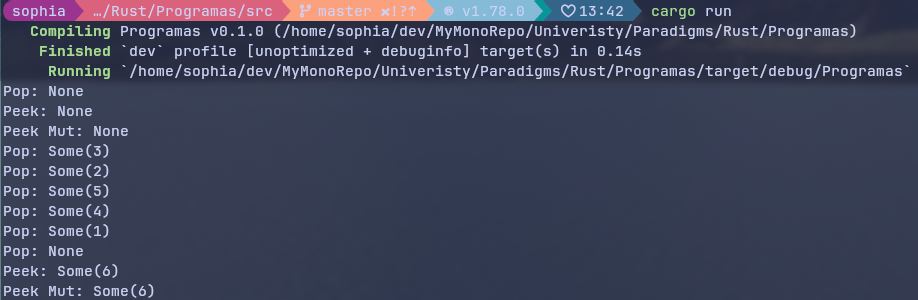
\includegraphics[scale=0.4]{ListRun}

Fonte: https://rust-unofficial.github.io/too-many-lists/

%%%--------------------------------------------------------------------
\section{Quick Sort}
%%%--------------------------------------------------------------------
  Organiza um vetor de n\'{u}meros usando o m\'{e}todo de parti\c{c}\~{a}o conhecido como quicksort

\begin{lstlisting}[language=rust]
quick.rs
extern crate std as core;

use core::cmp::Ordering;

fn quicksort_helper<T, F>
  (arr: &mut [T], left: isize, right: isize, compare: &F)
where F: Fn(&T, &T) -> Ordering {
    if right <= left {
        return
    }

    let mut i: isize = left - 1;
    let mut j: isize = right;
    let mut p: isize = i;
    let mut q: isize = j;

    unsafe {
        let v: *mut T = &mut arr[right as usize];
        loop {
            i += 1;
            while compare(&arr[i as usize], &*v) == Ordering::Less {
                i += 1
            }
            j -= 1;
            while compare(&*v, &arr[j as usize]) == Ordering::Less {
                if j == left {
                    break
                }
                j -= 1;
            }
            if i >= j {
                break
            }
            arr.swap(i as usize, j as usize);
            if compare(&arr[i as usize], &*v) == Ordering::Equal {
                p += 1;
                arr.swap(p as usize, i as usize)
            }
            if compare(&*v, &arr[j as usize]) == Ordering::Equal {
                q -= 1;
                arr.swap(j as usize, q as usize)
            }
        }
    }

    arr.swap(i as usize, right as usize);
    j = i - 1;
    i += 1;
    let mut k: isize = left;
    while k < p {
        arr.swap(k as usize, j as usize);
        k += 1;
        j -= 1;
        assert!(k < arr.len() as isize);
    }
    k = right - 1;
    while k > q {
        arr.swap(i as usize, k as usize);
        k -= 1;
        i += 1;
        assert!(k != 0);
    }

    quicksort_helper(arr, left, j, compare);
    quicksort_helper(arr, i, right, compare);
}
\end{lstlisting}

\begin{lstlisting}[language=rust]
pub fn quicksort_by<T, F>
  (arr: &mut [T], compare: F) where F: Fn(&T, &T) -> Ordering {
    if arr.len() <= 1 {
        return
    }

    let len = arr.len();
    quicksort_helper(arr, 0, (len - 1) as isize, &compare);
}

/// An in-place quicksort for ordered items.
#[inline]
pub fn quicksort<T>(arr: &mut [T]) where T: Ord {
    quicksort_by(arr, |a, b| a.cmp(b))
}
\end{lstlisting}
\newpage
\begin{lstlisting}[language=rust]
fn main() {
    let mut rng = rand::thread_rng();
    let len: usize = rng.gen();
    let mut v: Vec<isize> = rng.gen_iter::<isize>().take((len % 32) + 1).collect();
    for i in 0 .. v.len() - 1 {
        v[i] = v[i] % 1000;
    }
    quicksort(&mut v);
    println!("Unsorted:");
    for i in 0 .. v.len() - 1 {
        println!("{}", v[i])
    }
     println!("Sorted:");
    for i in 0 .. v.len() - 1 {
        println!("{}", v[i])
    }
}
\end{lstlisting}

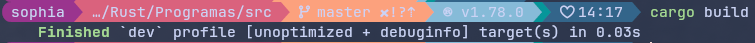
\includegraphics[scale=0.4]{QuickBuild}
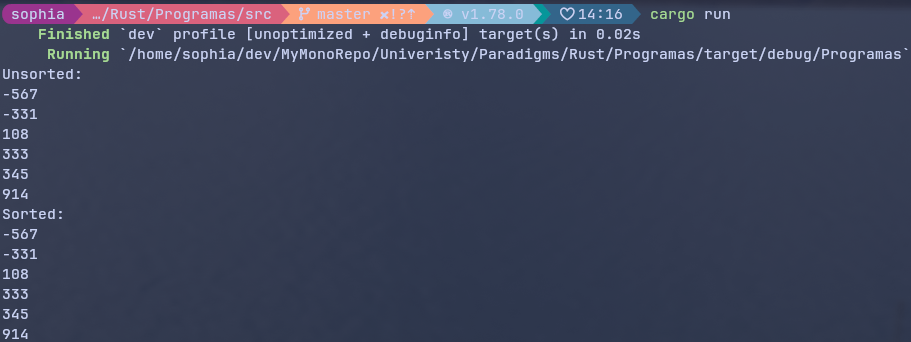
\includegraphics[scale=0.4]{QuickRun}

Fonte: http://www.cs.princeton.edu/~rs/talks/QuicksortIsOptimal.pdf

\pagebreak
\newpage
%%%--------------------------------------------------------------------
\section{IsPrime}
%%%--------------------------------------------------------------------
Verifica se um numero \'{e} primo

\begin{lstlisting}[language=rust]
prime.rs
fn main() {
    let num = 17;
    if is_prime(num) {
        println!("{} is prime", num);
    } else {
        println!("{} is not prime", num);
    }
}

fn is_prime(n: u32) -> bool {
    if n <= 1 {
        return false;
    }
    for i in 2..=n / 2 {
        if n % i == 0 {
            return false;
        }
    }
    true
}
\end{lstlisting}

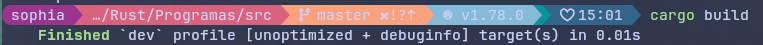
\includegraphics[scale=0.4]{PrimeBuild}
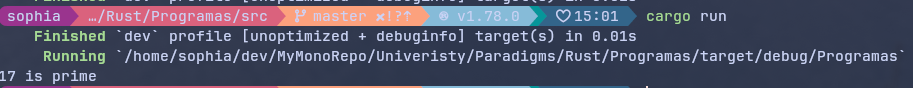
\includegraphics[scale=0.4]{PrimeRun}

Este c\'{o}digo \'{e} original deste livro
\pagebreak
\newpage

%%%--------------------------------------------------------------------
\section{Binary Search}
%%%--------------------------------------------------------------------
Verifica se um numero \'{e} primo

\begin{lstlisting}[language=rust]
binary.rs

fn main() {
    let arr = [1, 3, 5, 7, 9, 11, 13, 15, 17, 19];
    let target = 1;

    if let Some(index) = binary_search(&arr, target) {
        println!("Element {} found at index {}", target, index);
    } else {
        println!("Element {} not found in the array", target);
    }
}

fn binary_search(arr: &[i32], target: i32) -> Option<usize> {
    let mut left = 0;
    let mut right = arr.len() - 1;

    while left <= right {
        let mid = left + (right - left) / 2;
        if arr[mid] == target {
            return Some(mid);
        } else if arr[mid] < target {
            left = mid + 1;
        } else {
            right = mid - 1;
        }
    }
    None
}
\end{lstlisting}

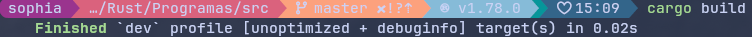
\includegraphics[scale=0.4]{BinaryBuild}
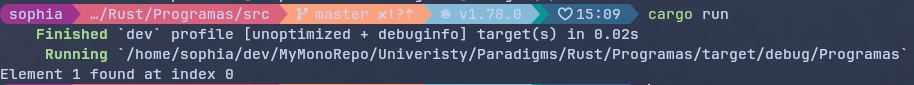
\includegraphics[scale=0.4]{BinaryRun}

Este c\'{o}digo \'{e} original deste livro
